% This is LLNCS.DEM the demonstration file of
% the LaTeX macro package from Springer-Verlag
% for Lecture Notes in Computer Science,
% version 2.2 for LaTeX2e
%
\documentclass{llncs}
%
\usepackage[german,american]{babel}
\usepackage[latin1]{inputenc}
% \usepackage{makeidx}  % allows for indexgeneration
\usepackage{graphicx}
\usepackage{epsfig}
\usepackage{hyperref}
\usepackage{moreverb}

%
\newcommand{\todo}[1]{\emph{[ToDo: #1]}}
%
\begin{document}

\title{DBpedia: Bootstrapping the Semantic Web}

\titlerunning{DBpedia}

\author{S\"oren Auer\inst{1,3} \and Chris Bizer\inst{2} \and Georgi Kobilarov\inst{2} \and Jens Lehmann\inst{1} \and Richard Cyganiak\inst{2} \and Zack Ives\inst{3}}

\authorrunning{S\"oren Auer et al.}

\tocauthor{S\"oren Auer (University of Pennsylvania),
Jens Lehmann (Universit\"at Leipzig)}
%
\institute{
Universit\"at Leipzig, Department of Computer Science, Johannisgasse 26,\\
D-04103 Leipzig, Germany,\\
\email{\{auer,lehmann\}@informatik.uni-leipzig.de}
\and
Freie Universit\"at Berlin, Web-based Systems Group, Garystr. 21,\\
D-14195 Berlin, Germany,\\
\email{\{bizer,kobilarov\}@wiwiss.fu-berlin.de, richard@cyganiak.de}
\and
University of Pennsylvania, Department of Computer and Information Science\\
Philadelphia, PA 19104, USA,\\
\email{auer@seas.upenn.edu}
}

\maketitle

\begin{abstract}
DBpedia is a community effort to extract structured information from Wikipedia
and to make this information available on the Web. DBpedia allows you to ask
sophisticated queries against datasets extracted from Wikipedia and to link other
datasets on the Web to Wikipedia data. We describe the extraction of the DBpedia
datasets, and how the resulting data can be made available on the Web for humans and
machines. We describe some emerging applications from the DBpedia community and describe how website operators can reduce costs by facilitating royalty-free DBpedia content within their sites. Finally, we present the current status of interlinking DBpedia with other open datasets on the web and outline how DBpedia could serve as a nucleus for a emerging Web of open data sources.
\end{abstract}

\section{Introduction}
\label{sec:introduction}

It is now almost universally acknowledged that stitching together the
world's structured information and knowledge to answer semantically
rich queries is one of the key challenges of computer science, and one
that is likely to have tremendous impact on the world as a whole.
This has led to almost 30 years of research into information
integration~\cite{multibase,DBLP:conf/sigmod/Wiederhold93} and
ultimately to the Semantic Web and related
technologies~\cite{p2p-mediation,hyperion,chatty-web}.  Such efforts
have generally only gained traction in relatively small and
specialized domains, where a closed ontology, vocabulary, or schema
could be agreed upon.  However, the broader goal of replacing the Web
is far from a reality, and one of the biggest challenges facing such
efforts has been how to get enough ``interesting'' and broadly useful
information into the system to make it useful and accessible to a
\emph{general} audience.  (For instance, there is only a limited
amount of RDF available, and few OWL ontologies are widely adopted.)

A challenge is that the traditional ``top-down'' model of designing an
ontology or schema \emph{before} developing the data breaks down at
the scale of the Web: both data and metadata must constantly evolve,
and they must serve many different communities.  Hence, there has been
a recent movement in building the Semantic Web grass-roots-style,
using incremental and Web 2.0-style collaborative
approaches~\cite{cidr-chasm,hyperion,orchestra-cidr,DBLP:journals/debu/DoanRCDLMSS06}.
Such a collaborative, grass-roots Semantic Web requires a new model of
structured information representation and management: first and
foremost, it must handle inconsistency, ambiguity, uncertainty, data
provenance~\cite{cui-thesis,DBLP:conf/icdt/BunemanKT01,DBLP:conf/vldb/BenjellounSHW06},
and implicit knowledge in a uniform way.

Perhaps the most effective way of spurring synergistic research along
these directions is to provide a rich corpus of diverse data.  This
would enable researchers to develop, compare, and evaluate different
extraction, reasoning, and uncertainty management techniques, and to
deploy operational systems on the Web.  Our goal is to develop such a
data resource, using the collaboratively edited Wikipedia
encyclopedia.  Wikipedia is heavily visited and under constant revision
(e.g., according to alexa.com, Wikipedia was the 11th most visited
website in the first quarter of 2007).  Wikipedia editions are
available in over 100 languages, with the English one accounting for
more than 1.7 million articles.  Like many other web applications,
Wikipedia has the problem that its search capabilities are limited to
full-text search, which only allows very limited access to this
valuable knowledge-base.  As has been highly publicized, Wikipedia
also exhibits many of the challenging properties of collaboratively
edited data: it has contradictory data, inconsistent taxonomical
conventions, errors, and even spam.

The DBpedia project focuses on the task of converting data from the
Wikipedia site into structured knowledge, such that Semantic Web
techniques can be employed against it --- asking sophisticated queries
against Wikipedia, linking to other datasets on the Web, or creating
new applications or mashups.  We make the following contributions:

\begin{itemize}

\item We develop a basic architecture for DBpedia extraction, which converts 
Wikipedia data to RDF and OWL.  The basic components form a foundation
upon which further research into information extraction, clustering,
uncertainty management, and query processing may be conducted.

\item We provide a basic RDF and OWL dataset, which can be used in a variety of Semantic 
Web applications.

\item We develop a series of interfaces and access modules, such that the dataset
can be accessed via Web services and linked to other sites.

\item We identify a research agenda for how Wikipedia data may be better exploited.

\end{itemize}

[Road map]


\section{Extraction Approaches}
\label{sec:extraction}

\begin{figure}
	\centering
	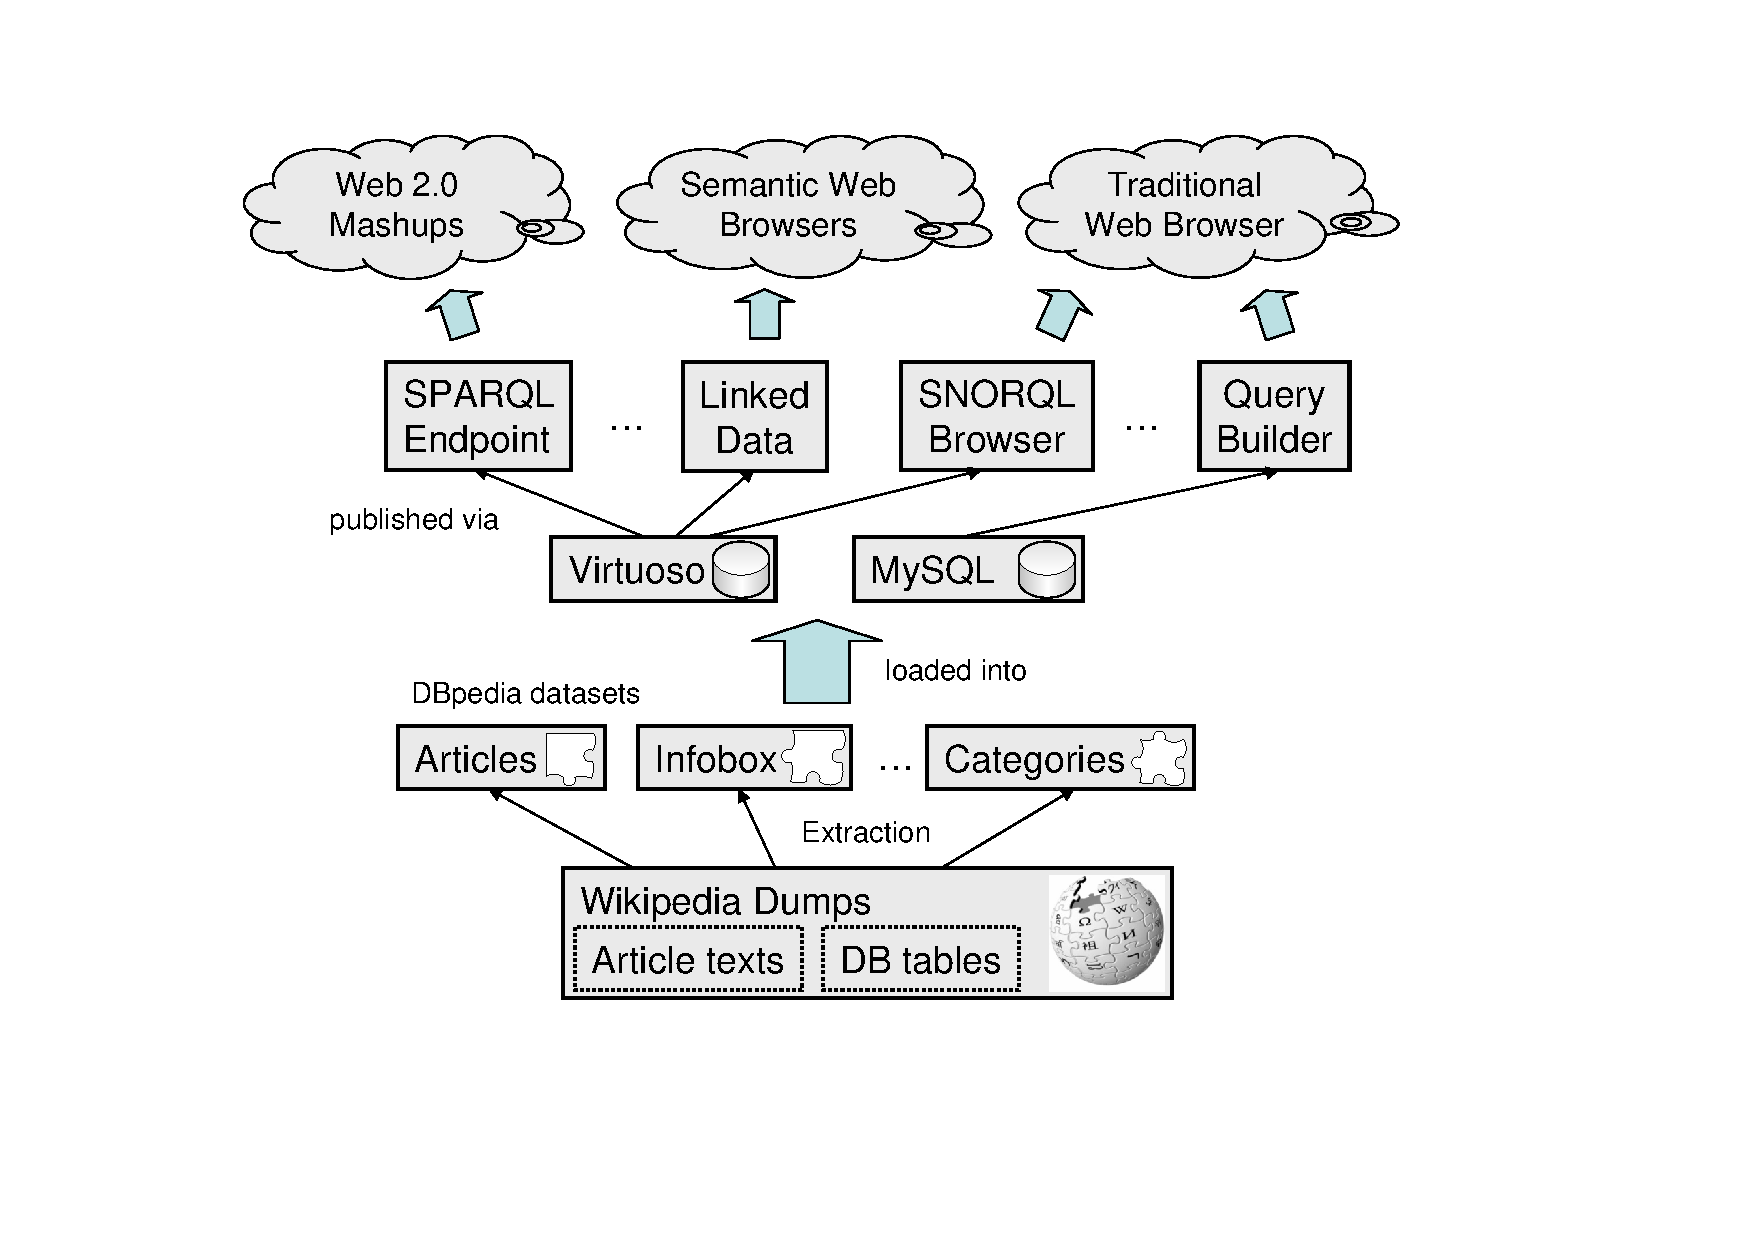
\includegraphics[width=0.70\textwidth]{architecture}
	\caption{DBpedia overview.}  \label{fig:architecture}
\end{figure}

Mediawiki\footnote{http://www.mediawiki.org} is the software used to run Wikipedia. Due to the nature of the Wiki system MediaWiki, basically all editing, linking, annotating with meta-data is done inside article texts by adding special syntactic constructs. Hence, most information can be obtained by parsing articles texts for these syntactic constructs. They include links (internal/external links, category links and links to other language versions), embedded images and templates.

Since Mediawiki exploits some of this information itself for rendering the user interface, some
information is additionally cached in relational database tables. Dumps of the crucial relational
database tables (including the ones containing the article texts) for the Wikipedia versions in
different languages are published on the Web on a regular
basis\footnote{http://download.wikimedia.org/}. Based on these Wikipedia database dumps, we
currently use two different methods of extracting and revealing semantic relationships:

\begin{itemize}
	\item Mapping of relationships already stored in relational database tables,
	\item Extraction of additional information directly from the article texts.
\end{itemize}

\todo{this needs further explanation}

\section{Classification of DBpedia data}

Wikipedia uses a category system to organize its articles. Some of these categories can be interpreted as OWL classes. The articles in such categories can then often be seen as instances of classes and subcategories are often subclasses. Unfortunately, the transition of the Wikipedia category hierarchy to a class hierarchy is not straightforward. Some categories serve only administrative purposes, others are more a "related-to" connection than an actual subsumption relation. The YAGO project \cite{suchanek2007WWW} tries to resolve this issue by linking Wikipedia leaf categories to WordNet concepts. However, there is still a need for a hierarchy which is more consistent with our extracted data sets and close to the Wikipedia category system. \emph{To be continued.}

\begin{itemize}
	\item Bachelor thesis in Leipzig
	\item Georgi and Nikos work based on YAGO classes. \emph{We should check whether we need a description of
YAGO here.}
\end{itemize}

\section{The DBpedia dataset}
\label{sec:dataset}

DBpedia currently provides information about more than 1.6 million 'things' (people, places,
objects, entities).  These things are described by around 91 million RDF triples, which have been
extracted from the English, German, French, Spanish, Italian, Portuguese, Polish, Swedish, Dutch,
Japanese and Chinese versions of Wikipedia. Todo: We need proper statistics here. Can be generated
with Virtuoso COUNT().

Table \ref{tab:DBpediaDatasets} gives an overview over the resulting datasets.

\begin{table}
	\centering
		\begin{tabular}{p{2.5cm}p{8cm}r}
			\textbf{Dataset} & \textbf{Description} & \textbf{Triples}\\
			\hline
\textit{Articles} & Descriptions of all 1.6 million concepts within the English Wikipedia including titles, short abstracts, thumbnails and links to the corresponding articles. & 5.4M \\
\textit{Extended Abstracts} & Additional, extended English abstracts. & 1.6M \\
 & Extended abstracts in 10 languages. & 1.3M \\
\textit{External Links} & Links to external web pages about a concept. & 2.8M \\
\textit{Article Categories} & Links from concepts to categories using the SKOS vocabulary. & 5.5M \\
\textit{Additional Languages} & Additional titles, short abstracts and Wikipedia article links in 10 languages. & 4.0M \\
\textit{Infoboxes} & Relationships between concepts and data attributes for concepts that have been extracted from infoboxes. & 9.1M \\
\textit{Categories} & Information which concept is a category and how categories are related. & 0.9M \\
\textit{Persons} & Information about 58,880 persons (date and place of birth etc.) represented using the FOAF vocabulary. & 0.4M\\
\textit{Geonames Links} & Links between geographic places in DBpedia and data about them in the Geonames database. & 0.2M \\
\textit{Location Types} & \verb|rdf:type| Statements for geographic locations obtained from the Geonames database. & 65K \\
\textit{DBLP Links} & Links between computer scientists in DBpedia and their publications in the DBLP database. & 200\\
\textit{RDF Book Mashup Links} & Links between books in DBpedia and data about them provided by the RDF Book Mashup. & 9K \\
\textit{PageLinks} & Internal links between DBpedia instances derived from the internal pagelinks between Wikipedia articles. & 60M \\
		\end{tabular}
	\caption{DBpedia datasets}
	\label{tab:DBpediaDatasets}
\end{table}

Some datasets (such as the \textit{Persons} or \textit{Infoboxes} datasets) are semantically rich in the sense that they contain very specific information. Others (such as the \textit{PageLinks} dataset) contain meta-data (such as links between articles) without a specific semantics.

\begin{figure}[tbp]
\begin{minipage}[b]{.53\linewidth} 
\fontsize{9pt}{0}
\begin{listing}{1}
{{Infobox Town AT |
  name = Innsbruck |
  image_coa =  InnsbruckWappen.png |
  image_map = Karte-tirol-I.png |
  state = [[Tyrol]] |
  regbzk = [[Statutory city]] |
  population = 117,342 |
  population_as_of = 2006 |
  pop_dens = 1,119 |
  area = 104.91 |
  elevation = 574 |
  lat_deg = 47 |
  lat_min = 16 |
  lat_hem = N |
  lon_deg = 11 |
  lon_min = 23 |
  lon_hem = E |
  postal_code = 6010-6080 |
  area_code = 0512 |
  licence = I |
  mayor = Hilde Zach |
  website = [http://innsbruck.at] |
}}
\end{listing}
\vspace{2pt}
%\caption{Wikipedia template}
\end{minipage}
\hspace{.03\linewidth}
\begin{minipage}[b]{.42\linewidth}
\centering
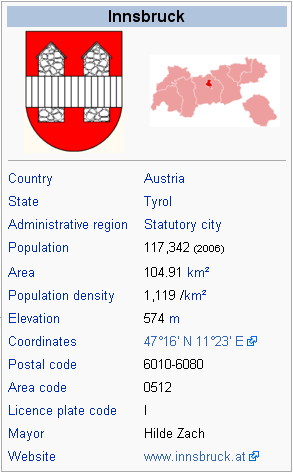
\includegraphics[width=\textwidth]{innsbruck}
%\caption{rendered output}
\end{minipage}
% hier koennte man auch eine gemeinsame Bildunterschrift angeben, wenn gewuenscht
\caption{Example of a Wikipedia template and rendered MediaWiki output.}
\label{fig:template}
\end{figure}

Figure \ref{fig:template} shows the template and rendered output of the Austrian town Innsbruck \emph{[ToDo: this example is from our ESWC 2007 paper -- it should be replaced by a different one]}. The infobox extraction algorithm detects such templates and recognizes their structure using pattern matching techniques. It selects significant templates, which are then parsed and transformed to RDF triples. The algorithm uses postprocessing techniques to increase the quality of extraction. MediaWiki links are recognized and transformed to suitable URIs, common units are detected and transformed to datatypes. Furthermore, the algorithm can detect lists of objects, which are transformed to RDF lists. Details about the infobox extraction algorithm can be found in \cite{DBLP:conf/esws/AuerL07}.

All extraction algorithms are available as Open-Source software\footnote{\url{http://sf.net/projects/dbpedia}}.


\section{Accessing the DBpedia Dataset}

The DBpedia dataset is published under GNU Free Documentation License, which allows information consumers to use the data, including the abstracts royalty-free.

The Dbpedia dataset is served using three publication mechanisms: SPARQL Endpoint, Linked Data and Dump

\subsection{SPARQL Endpoint}

Due to continued maturation of Semantic Web technologies there are meanwhile a number of toolkits available, which are able to handle large amounts of RDF data. For a publicly accessible RDF knowledge base such as DBpedia, however, there are a number of additional challenges:

\begin{itemize}
	\item Queries should run reasonably fast or warnings should be issued.
	\item Multiple applications should be able to query concurrently without interfering each other.
\end{itemize}

The DBpedia SPARQL endpoint is hosted using the Virtuoso Universal Server\footnote{http://virtuoso.openlinksw.com}.

\subsection{Linked Data Interface}

The DBpedia dataset is also served as Linked Data\cite{TimLinkedData}. 

The DBpedia dataset is served as Linked Data meaning that all DBpedia URIs are dereferencable. This allows you to browse the DBpedia dataset with Semantic Web browsers like Disco, Tabulator, the OpenLink Data Web Browser or Objectviewer.


\subsection{Database Dump}

The current extraction set is about 1.8 GB of zipped files (about 7.5 GB unzipped).
This access model can be used by sites and applications that are interested in larger parts of the dataset.
 
\subsection{Interlinking DBpedia with other Datasets}

DBpedia is the first project chosen for showcasing by the Linking Open Data\footnote{http://esw.w3.org/topic/SweoIG/TaskForces/CommunityProjects/LinkingOpenData} community of the Semantic Web Education and Outreach (SWEO) interest group within the W3C. That community has committed to make portions of other massive data sets, such as the US Census, Geonames, MusicBrainz, WordNet, the DBLP bibliography and many others, interoperable as well.


In addition to the DBpedia endpoint, we have increasingly many datasources in the Web 2.0 style, such as XML, RSS, JSON feeds or SPARQL end-points (e.g. see Programmableweb\footnote{\url{http://programmableweb.com}} for a comprehensive list). Integrating and combining such data sources still requires manual efforts (e.g. programming "mashups").

\begin{figure}[h]
	\centering
		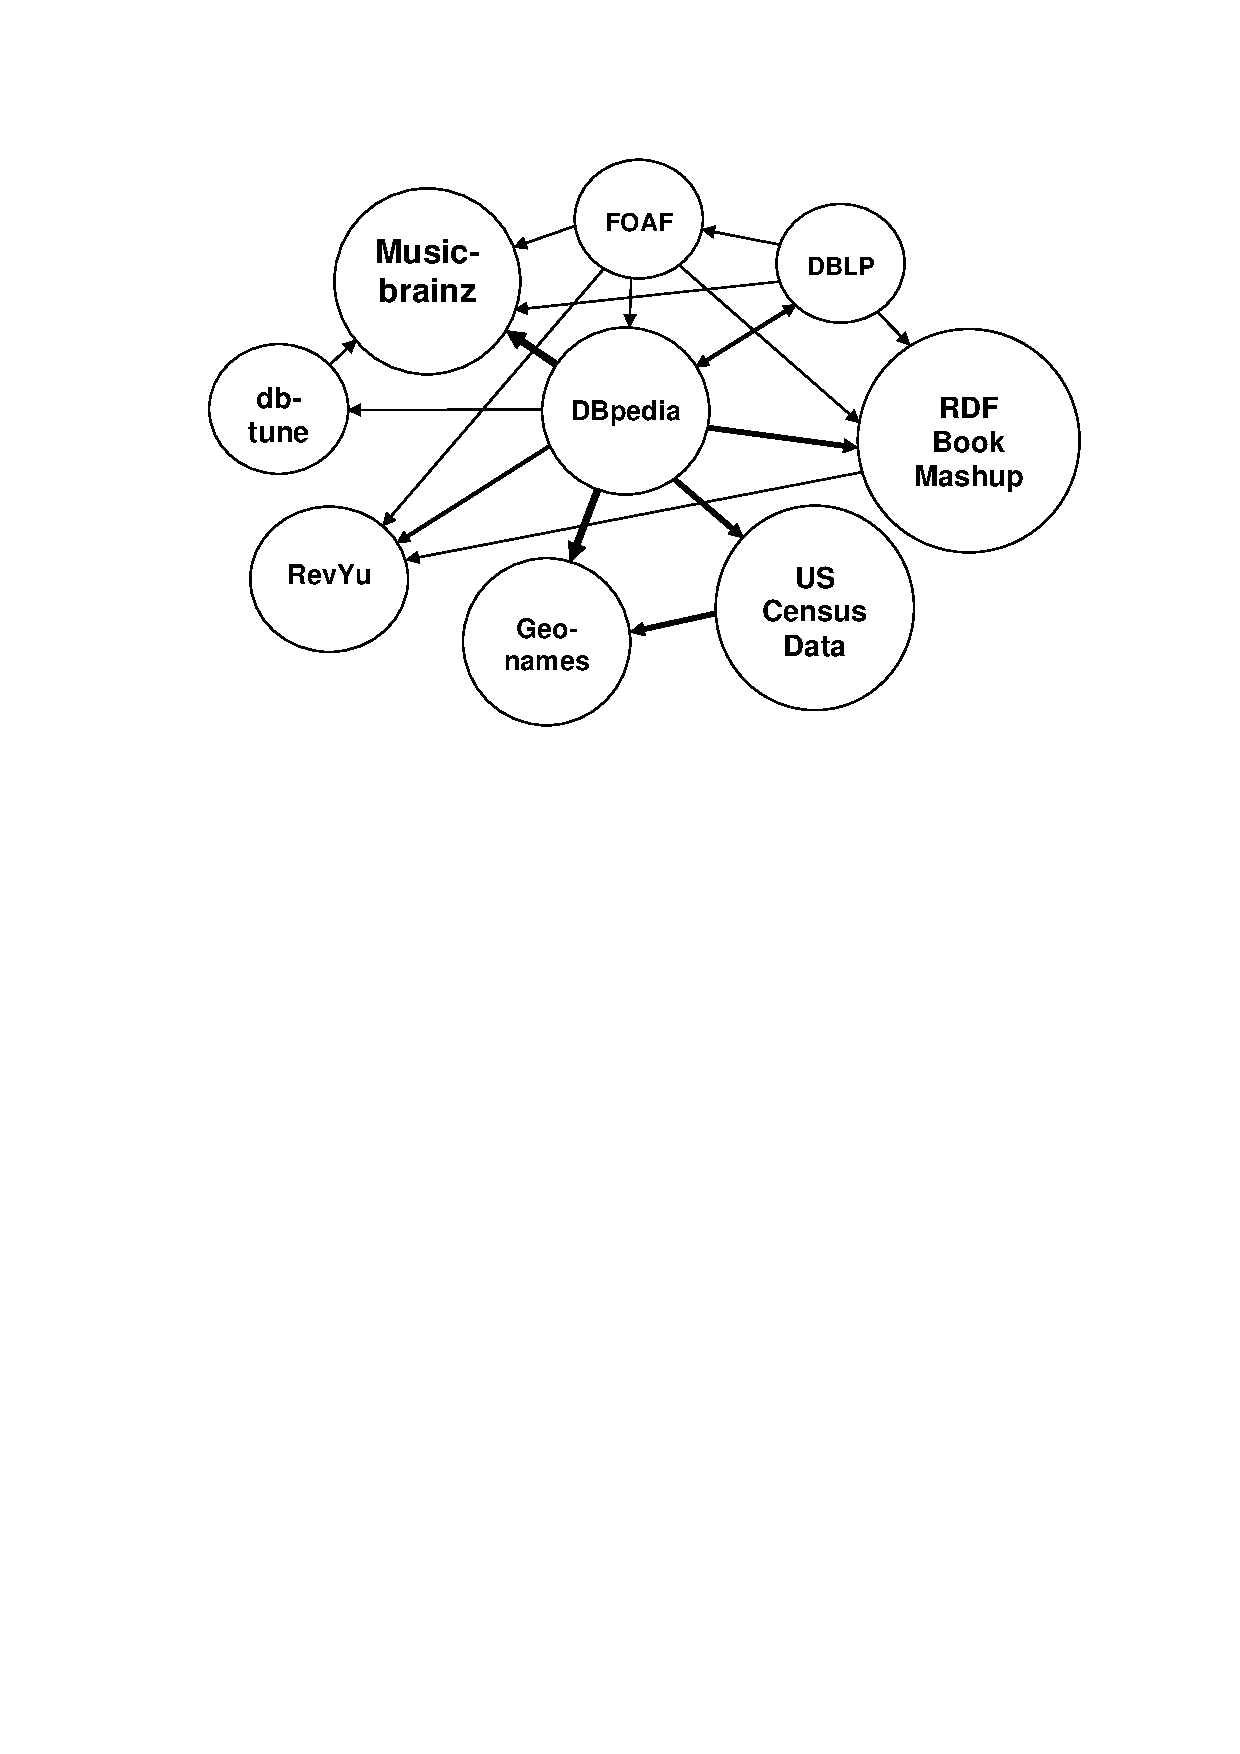
\includegraphics[width=0.90\textwidth]{Firgure1.pdf}
	\caption{Datsets that are interlinked with DBpedia}
	\label{fig:Firgure1}
\end{figure}

\subsubsection{Out-bound Links}

Talk about different datasets that are interlinked with DBpedia. Talk about record linkage
algorithms that are used.

As geographic places appear in Wikipedia as well as in the Geonames database, it is possible to use a heuristic to match instances from both datasources. The geonames web service uses such a heuristic to infer links to Wikipedia. The heuristic is based on the article title together with semantic information like latitude and longitude, but also country, administrative division, feature type, population and categories which is scraped from the Wikipedia articles. Marc from Geonames has send us 70500 resulting correspondences \todo{imho this sounds too informal for an ISWC paper (Jens)} which we use to auto-generate owl:sameAs links between cities in DBpedia and cities in Geonames. An example link is shown below: 

\begin{verbatim*}
<http://DBpedia.org/resource/Berlin> owl:sameAs <http://sws.geonames.org/2950159>
\end{verbatim*}

\subsubsection{In-bound Links}

DBpedia URIs can also be used to express your interests within your FOAF profile.

\begin{verbatim*}
<http://richard.cyganiak.de/foaf.rdf#cygri> foaf:topic_interest <http://DBpedia.org/resource/Semantic_Web> .
\end{verbatim*}

Another use case for DBpedia URIs could be to categorize blog posts or other documents. The advantage of this approach is that all DBpedia URIs are backed with data and thus allow clients to retrieve more information about a topic.

\begin{verbatim*}
<http://news.cnn.com/item1143> dc:subject <http://DBpedia.org/resource/Iraq_War> .
\end{verbatim*}

\section{Light-weight information and application integration}

In addition to establish simple links between data sources (as explained in the last Section), the ultimate goal of DBpedia is to contribute to a tight information and application integration on the Web. This is very related to the Web Services and Semantic Web Services initiatives. However, the understanding of Web Services within the research community (solely focusing on SOAP, WSDL, UDDI) meanwhile slightly differs from the Web Services actually deployed in a global scale. These are light-weight Web-API's, which can be accessed following the AJAX and JSON, REST paradigms. The website Programmableweb.com for example lists over 408 public and globally accessible information sources and web accesible applications and new ones are added daily.

We see DBpedia at the core of achieving a semantic integration of these light-weight Web services for two reasons. First, DBpedia provides huge multi-domain ontology, which can effectively used to align inputs and output definitions. Second, DBpedia itself provides an enormous knowledge source for the generation of a multiplicity of specialized light-weight information sources. What are the steps required to achieve this vision:

%Solution: Develop a (formal) model and Web application scenario which will enable semi-automatic integration, combination, aggregation (orchestration?) of such light-weight distributed data source.

\begin{itemize}
	\item Enable self-description of data and information sources -- such as the \verb|index.html| page for a web-site on a web-server. A special RDF vocabulary could serve this purpose. For the sake of simplicity, this vocabulary should be easily mappable into JSON.
	\item Allow server side views in the fashion of stored procedures or prepared statements. Such server side views can be simple, parametrized SPARQL\cite{sparql} queries with placeholders.
	\item Parameters (i.e. inputs) and return values (i.e. outputs) of such server provided views should be described semantically. For example, RDF class identifiers (URIs) can be used for annotating inputs and outputs.
\end{itemize}

Combined, this will enable end-user driven web-scale data integration in the way that information sources can be (semi-automatically) combined by aligning outputs of one information source to the inputs of another. The creation of `semantic Mashups' based on these self-describing information sources will not require any programming.


\section{User-Interfaces}

User-Interfaces for DBpedia can range from a simple table within a classic webpage, over browsing-based interfaces to different types of query interfaces.

%Hence, within the DBpedia project we aim to provide a number of different query and browse facilities for exploring the DBpedia datasets.

\subsection{Simple Integration of DBpedia Data into Web Pages}

Talk about potential for website maintainers (free content, tables that automatically update). Talk about Niko's examples (cities table, bands). 

A nice thing about Wikipeda is that it is kept up-to-date by a large community. Therefore, if you need a table on your webpage with let's say German cities, African musicians, Amiga computer games 
%from the 90ies 
or whatever you could generate this table with a SPARQL query against the DBpedia endpoint and your table will stay up-to-date as Wikipedia changes. Such tables can either be implemented using Javascript on the client or with a scripting language like PHP on the server. The second option also allows you to cache query results. 

Talk about reintegrating tables into Wikipedia??

Talk about Exhibit.

Talk about iSPARQL dynamic pages??

\subsection{Browsing DBpedia Data}

The DBpedia dataset is served as Linked Data meaning that all DBpedia URIs are dereferencable. This allows you to browse the DBpedia dataset with Semantic Web browsers like Disco, Tabulator, the OpenLink Data Web Browser or Objectviewer.
\todo{this is already in the Linked Data Interface section (Jens)}


\subsection{DBpedia Search}
In contrast to common full text search, structured data offers the opportunity to benefit from entities relations. 
Instead of forcing the user to guess keywords and the website admin to anticipate that guess, structured search brings up the possibility of stepwise narrowing the resultset in different dimensions. Unlike generic faceted browsing approaches, DBpedia Search was meant to fit inherent structure of the DBpedia dataset. The approach is nonetheless applicable to later scale. It enables the user to explore the data by entering a neighborhood of what he is looking for and narrowing and browsing the resultset.

Like common search engines, search session start with a keyword search. But the resultset will be calculated using also the semantic rich relations between entities. So are all results included and firstly shown to the user that fits the keywords or are related to these keyword-results by up to two steps.
A search for "`Scorsese"' will include the director Martin Scorsese, all of his films and the actors of these films.

The DBpedia dataset as an enclosed data space allows using similar weighting mechanisms like web search engines, namely page links. Sampling showed that overall important articles in Wikipedia receive more page links from other articles than less imported. So we chose to use a combination of page link count and relation depth to calculated search result relevance values.

The so generated resultset of direct full text results and related results is now used to build a tag cloud of the classes of all included entities using the classification approaches described in xx. Each class weight is itself calculated from the associated result weight and the frequency of occurrence. This tag cloud enables the user to narrow the resultset to a specific type of entities, which is only related to the former keyword search. In addition an extension is conceivable, where the user could further use a similar cloud mechanism to get shown the relations between results.

To view all properties of a DBpedia entity there is a details view, which is adjusted to fit the DBpedia dataset. Furthermore all outbound-links are followed and the retrieved data is shown together with the DBpedia data.

This should be an example of an both simply useable and also useful search interface using semantic rich data.


\subsection{Querying DBpedia Data}

Talk about Georgie's free text search, browse, tag cloud, other datasets interface.

Compared to most of the other Semantic Web knowledge bases currently available, for the RDF extracted from Wikipedia we have to deal with a different type of knowledge structure \--- we have a very large information schema and a considerable amount of data adhering to this schema. Existing tools unfortunately mostly focus on either one of both parts of a knowledge base being large, schema \textit{or} data.

If we have a large data set and large data schema, elaborated RDF stores with integrated query engines alone are not very helpful. Due to the large data schema, users can hardly know which properties and identifiers are used in the knowledge base and hence can be used for querying. Consequently, users have to be guided when building queries and reasonable alternatives should be suggested.

We specifically developed a graph pattern builder for querying the extracted Wikipedia content. Users query the knowledge base by means of a graph pattern consisting of multiple triple patterns. For each triple pattern three form fields capture variables, identifiers or filters for subject, predicate and object of a triple. While users type identifier names into one of the form fields, a look-ahead search proposes suitable options. These are obtained not just by looking for matching identifiers but by executing the currently built query using a variable for the currently edited identifier and filtering the results returned for this variable for matches starting with the search string the user supplied. This method ensures, that the identifier proposed is really used in conjunction with the graph pattern under construction and that the query actually returns results. In addition, the identifier search results are ordered by usage number, showing commonly used identifiers first. All this is executed in the background, using the Web 2.0 AJAX technology and hence completely transparent for the user. Figure \ref{fig:querybuilder} shows a screenshot of the graph pattern builder.

\begin{figure}[htbp]
	\centering
		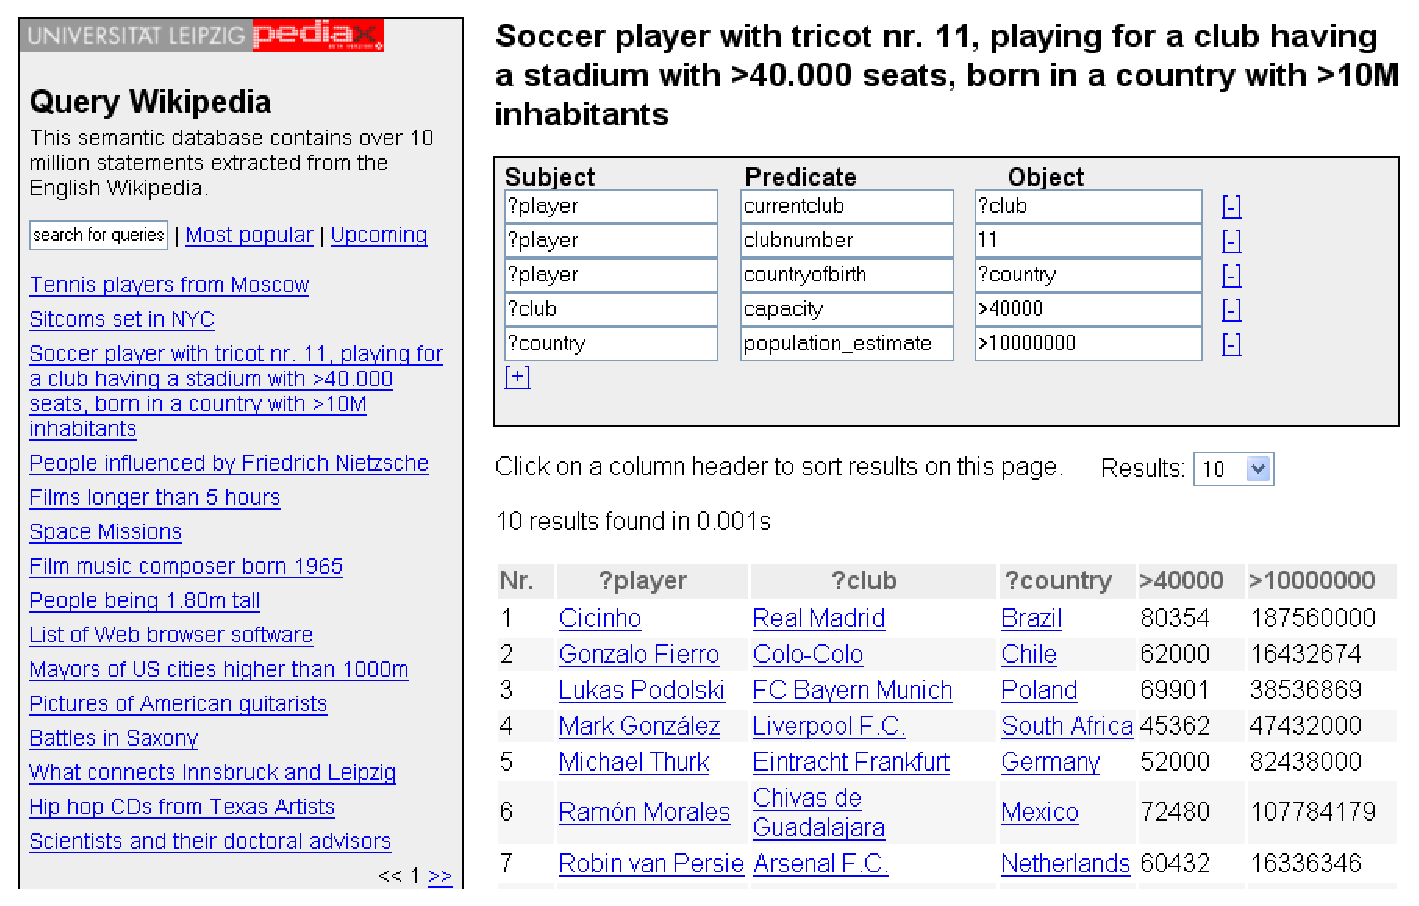
\includegraphics[width=0.80\columnwidth]{querybuilder}
	\caption{Form based query builder}
	\label{fig:querybuilder}
\end{figure}

Talk about SNORQL query explorer.

Talk about Virtuoso SPARQL query builder.

\subsubsection*{DBpedia Object Connector}

\emph{[The DBpedia object connector is currently under construction. (Jens)]}
The DBpedia instance data can be seen as a huge RDF graph, where objects are connected by properties. An interesting application of our DBpedia data set is to answer the question what two objects have in common. This question can be answered by computing the shortest path between two objects in the DBpedia Infobox RDF graph. In our search for efficient solutions for this problem, we found interesting structural properties of Wikipedia: The RDF graph cannot be easily decomposed in subgraphs, i.e.~a large fraction of the articles belong to the same subgraph. This hold true even if we remove all category connections (including articles describing categories). This indicates that Wikipedia infoboxes are deeply interlinked -- often across several domains. The connections between different objects are not always obvious. In fact, the shortest path between two objects can have a length of up to approximately 20.000. The DBpedia object connector can reveal interesting and often surprising connections, which are unlikely to be found by any other application. \todo{show a screenshot with an interesting example; hopefully the data connector will be finished in time (Jens)}

\subsection{Domain-specific User Inferfaces}

The DBpedia project aims at providing a hotbed for applications and mashups based on information from Wikipedia. Although DBpedia was just recently launched, a number of 3rd party applications is already available.

The Java WikiStory \ref{fig:wikistory} enables users to browse Wikipedia articles about people on a large timeline.

\begin{figure}
	\centering
		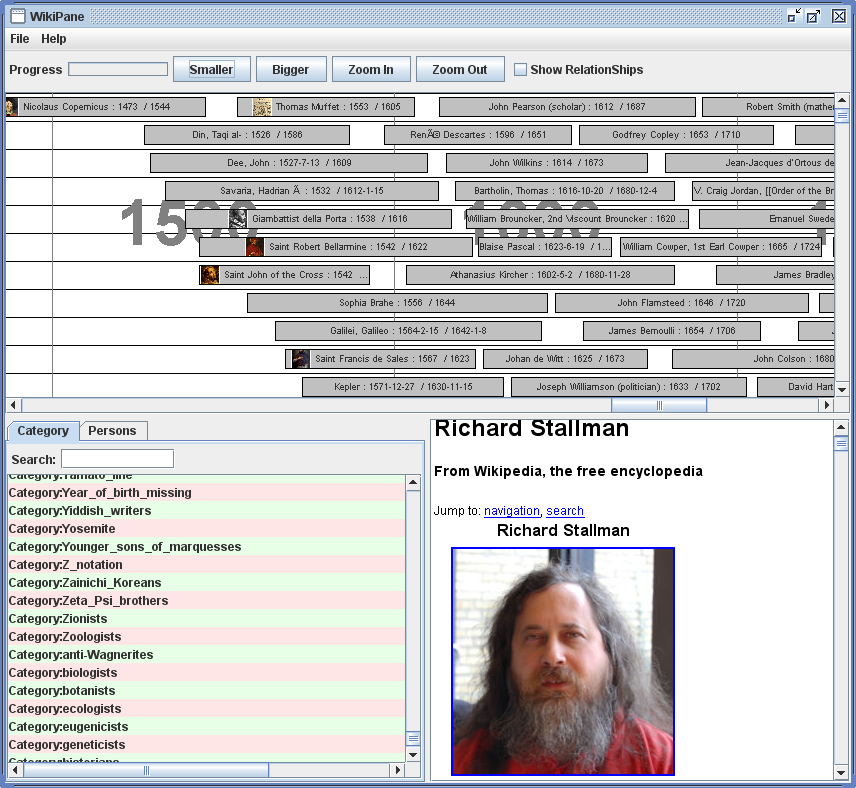
\includegraphics[width=0.50\columnwidth]{wikistory}
	\caption{WikiStory}
	\label{fig:wikistory}
\end{figure}

Talk about Objectseet, spreadsheet application.

\section{Related Work}

Talk about relation to Freebase.

Talk about relation to this commercial Wikipedia clone.

Talk about relation to Semantic Media Wiki. Potential synergies.

YAGO \cite{suchanek2007WWW} extracts exactly 14 relations, such as subClassOf, type, familyNameOf, locatedIn from different sources. One source is the Wikipedia category system (for subClassOf, locatedIn, diedInYear, bornInYear), and another one are Wikipedia redirects (means relation). YAGO does not perform an infobox extraction as in our approach. For determining (sub)class relationships, YAGO does not use the Wikipedia category hierarchy. Instead, they only consider the leaf categories and link them into the WordNet hierarchy.

Find the other papers on Wikipedia info extraction and talk about them.

\section{Conclusions}

DBpedia is a mayor source of open, royalty-free data on the Web. By interlinking it with further data sources, it could serve as a nucleus for the emerging Web of Open data sources.

Talk about future plans.

\section*{Acknowledgments}
We are grateful to the members of the growing DBpedia community, who are actively contributing to the project. In particular we would like to thank the splendid OpenLink team around Kingsley Idehen and Orri Erling.
%This research was supported in part by the following grants: BMBF (SE2006 \#01ISF02B), NSF (SEIII
%\#IIS-0513778). We are grateful to J\"org Sch\"uppel, who participated in the implementation of the
%extraction algorithm, and the anonymous reviewers for their suggestions.

\bibliographystyle{plain}
\bibliography{SoerenAuer,New,zives-short}

\emph{[Page Limit: 14 pages]}

\end{document}